\documentclass[11pt]{article}
\usepackage[letterpaper,margin=1in]{geometry}
\usepackage[T1]{fontenc}
\usepackage{lmodern,microtype,amsmath,amssymb}
\usepackage{booktabs,tabularx,array,graphicx,caption}
\usepackage{enumitem,titlesec}
\usepackage[hidelinks]{hyperref}
\usepackage{xurl}
\usepackage{float}
\newcolumntype{Y}{>{\raggedright\arraybackslash}X}
\setlength{\parindent}{0pt}
\setlength{\parskip}{0.5em}
\setlist{nosep,leftmargin=1.4em}
\renewcommand{\arraystretch}{1.12}
\captionsetup{font=small,labelfont=bf}
\titleformat{\section}{\large\bfseries}{\thesection}{0.6em}{}
\titleformat{\subsection}{\normalsize\bfseries}{\thesubsection}{0.5em}{}
\graphicspath{{figures/}}

\title{\vspace{-2em}\textbf{Agricultural Risk Management \& Weather Derivative Replicating Platform}\\[0.3em]
\large ECE 473 / COS 473 --- Milestone II: Contract Design \& Platform Architecture}
\author{Maya, Evan, Jack}
\date{November 2026}

\begin{document}
\maketitle

\section*{Executive Summary}

\textbf{Showcase: the PRF Companion.} A working web app that keeps a rancher's USDA rainfall insurance and
uses Kalshi contracts to cover the months it leaves open. It tests each month at the rancher's location,
recommends only the months that track, and builds the order. Fit on 1951--2000 and scored on 2001--2025,
the companion has a median hedge effectiveness of 0.61, against 0.23 for hedging the PRF intervals themselves.
It is recommended for 9 of our 11 farms (Section~4).

Milestone I measured how far today's Kalshi monthly-rain contracts are from USDA's Pasture, Rangeland
and Forage (PRF) rainfall-index insurance. Milestone II builds the tools the proposal promised and uses
them to answer two questions: \emph{what is the best hedge a farmer can buy}, and \emph{what would have to
change for it to be good}. All results use the 11 representative farms at our 7 PRF study sites, their
2026 PRF elections, and the NCEI-based PRF index that PRF pays on from crop year 2027, over 1951--2025.
Hedge effectiveness (HE) is the share of the year-to-year variance of the farm's PRF payout that a hedge
removes. We report it \emph{out of sample}: the hedge is refit 75 times, leaving out one year each time,
and scored on the year it did not see.

\begin{enumerate}
  \item \textbf{Optimizer (Week 4, Jack).} A convex program that picks the lowest-error portfolio of Kalshi
  contracts for any budget, with prices, fees, capital cost and order-book depth. The cheapest hedge with
  90\% of the best fit costs 22\% less than the lowest-error hedge and loses nothing out of sample.
  \item \textbf{Error breakdown (Week 4, Maya).} Out of sample, HE falls from 1.00 to 0.17:
  geography $-0.35$, settlement source $-0.13$, monthly contracts $-0.19$, whole-inch strikes $\approx 0$,
  order-book depth $-0.16$, and a budget equal to the PRF premium $-0.01$.
  \item \textbf{Contract gaps and proposals (Week 4, Evan).} Only 3 of 36 insured windows replicate well
  today; summer convective and monsoon rain fails everywhere. Two-month contracts raise pooled HE from
  0.34 to 0.48; binaries on the PRF grid index itself reach 0.98, but that is PRF without the subsidy.
  \item \textbf{Platform (Week 5, Jack and Maya).} A working web app: a farmer clicks a location, picks any
  months, and gets an order ticket priced from live Kalshi order books where markets are listed, a
  price-vs-fit frontier, a 75-year backtest, and a comparison with PRF.
  \item \textbf{Complementing PRF (refinements promised in our Milestone I update).} The best niche is the
  months PRF leaves uncovered: single-month cover for November--February copies about half of the payout
  swings (median HE 0.52; December 0.68). A top-up above PRF's 90\% cap copies little (0.14). Excess-rain
  cover needs two-month contracts (0.22 to 0.40). Backtests on the CPC index USDA actually paid tell the same story.
  \item \textbf{App test (Week 5, Evan).} Typing the 11 farms into the app reproduces the analysis exactly. The
  recommended hedges cost 1.71$\times$ the farmers' PRF premiums (median) and copy a bit over a third of PRF's
  payout swings out of sample (median HE 0.38). Across 150 random grids the median HE is 0.47 within 25 miles
  of a station and 0.15 beyond 100 miles; 69\% of sampled grids score below 0.3.
  \item \textbf{Showcase: PRF Companion.} Built on these results; see Section~4.
\end{enumerate}

%=====================================================================
\section{Designing Better Options (Week 4)}

\subsection{Lowest-error, lowest-cost portfolios (Jack)}

\textbf{Problem.} In year $t$ the farmer wants $y_t$ dollars (the PRF indemnity). A \emph{leg} is a NO
contract on ``station rain in month $m$ above $K$ inches'', paying \$1 if rain $\le K$. Each leg can be
bought in \emph{tranches}: price levels of an order book with sizes, or an unlimited quantity at a model
price. With $x_j$ contracts in tranche $j$, all-in unit cost $c_j$ and hedge payout $h_t$,
\[
\min_{x}\ \frac1n\sum_t (y_t-h_t)^2 \quad\text{s.t.}\quad \sum_j c_j x_j \le B,\qquad 0\le x_j\le \text{cap}_j ,
\]
where $c_j = (p_j + 0.07\,p_j(1-p_j))(1 + r\,d/365)$ adds Kalshi's taker fee and the cost of prepaying
cash ($r=4.05\%$, $d=31$ days). We solve the penalized form with L-BFGS-B and find the budget form by
bisection on the penalty. Sweeping $B$ traces the \emph{efficient frontier}. With $B=\infty$ and no caps it
reproduces Milestone I's least-squares hedge exactly.

\begin{figure}[H]\centering
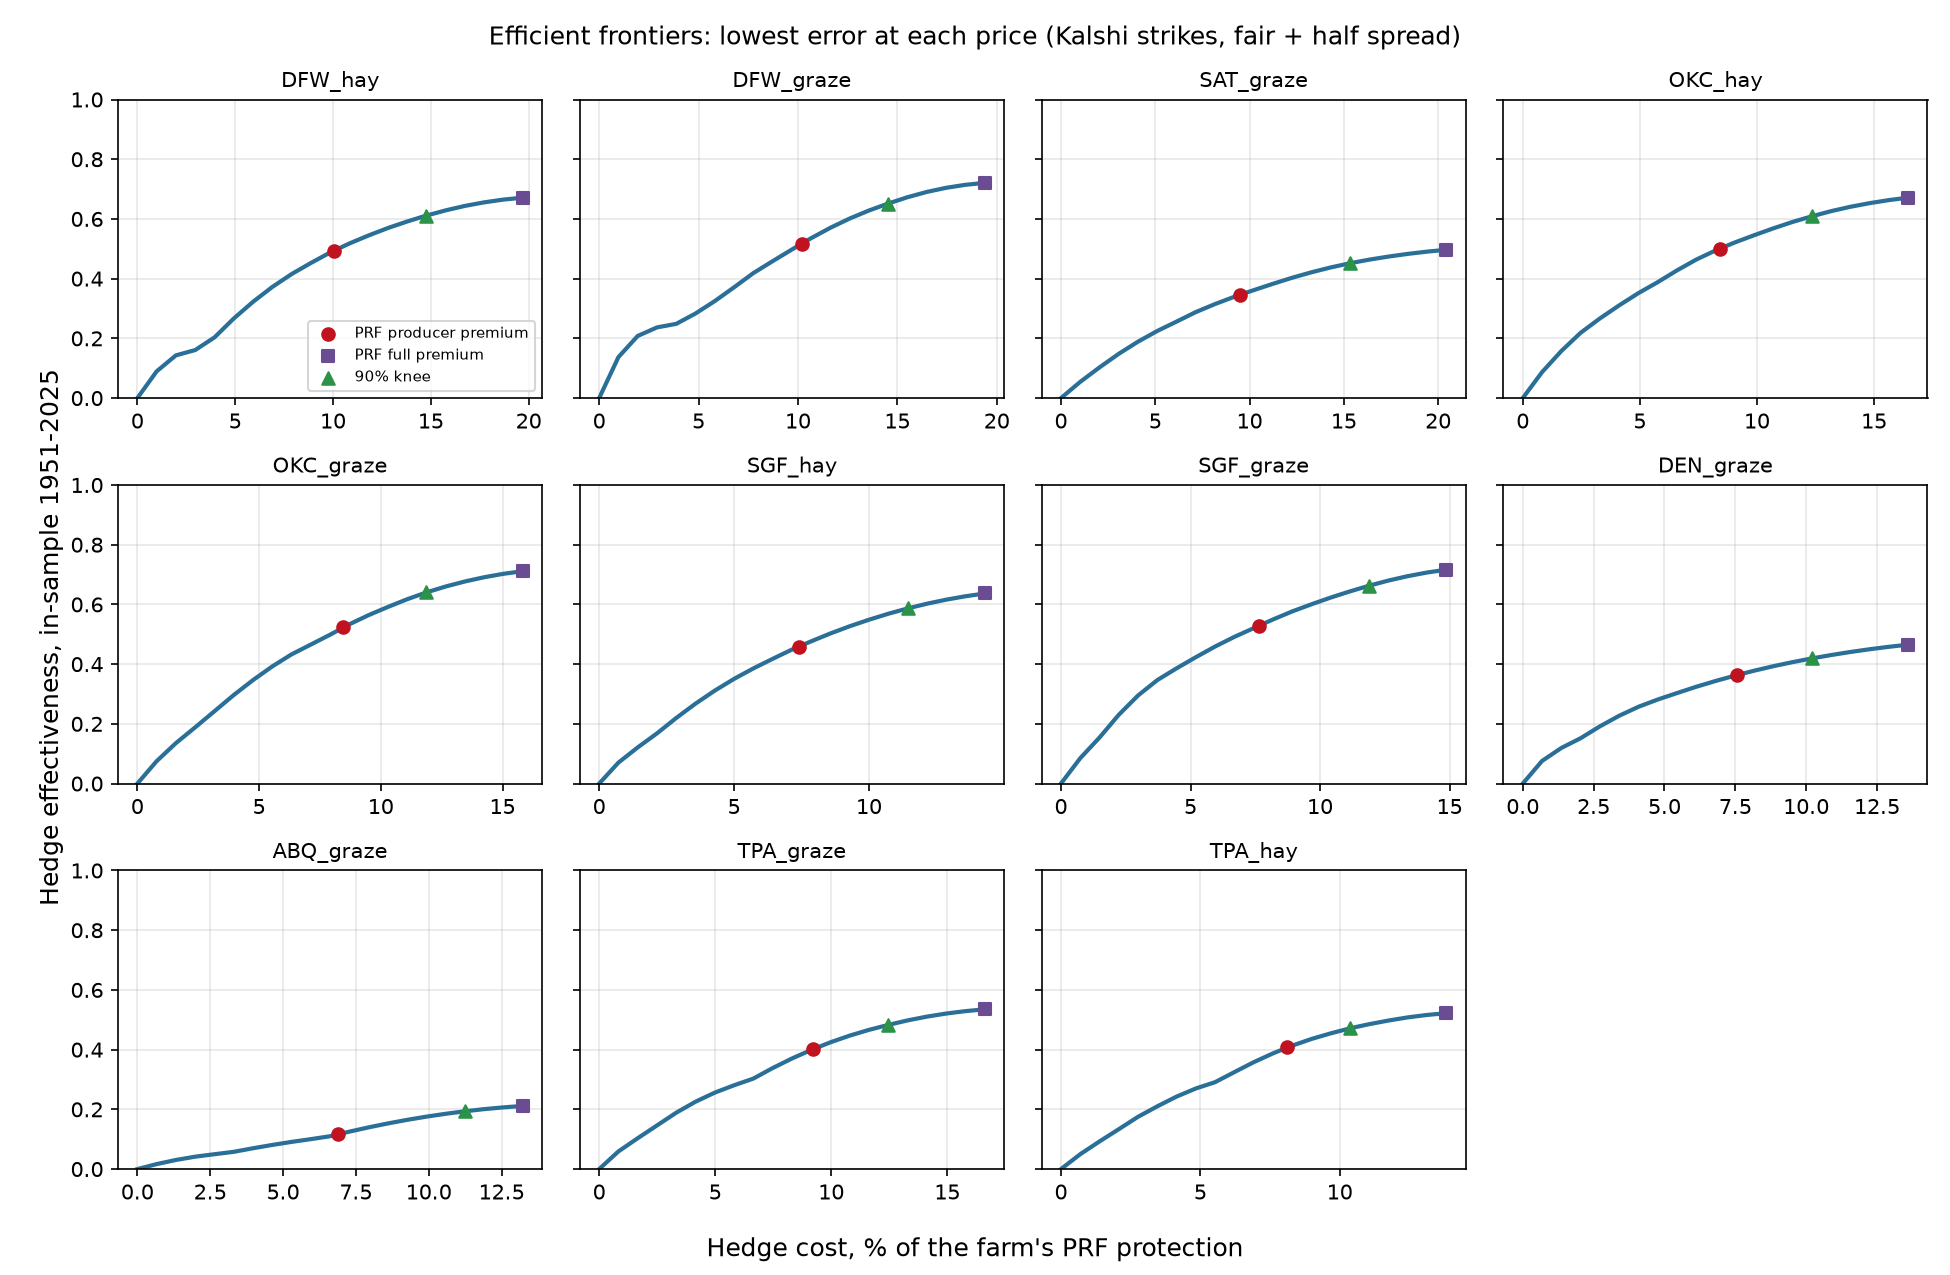
\includegraphics[width=\textwidth]{m2_frontiers.png}
\caption{Efficient frontiers for the 11 farms (in-sample HE vs.\ cost as \% of PRF protection). Red: budget
equal to the farm's PRF producer premium. Green: the ``90\% knee''. Purple: full PRF premium.}
\end{figure}

\begin{table}[H]\centering\small
\begin{tabularx}{\textwidth}{Yrrrr}
\toprule
Point on the frontier (11 farms) & Cost / yr & \$ per \$1 expected & Median HE in & Median HE out \\
\midrule
Lowest error (no budget) & \$104,970 & 1.10 & 0.64 & 0.37 \\
90\% knee & \$81,516 & 1.11 & 0.59 & 0.36 \\
Budget = PRF producer premium & \$55,992 & 1.12 & 0.46 & 0.30 \\
\midrule
PRF itself: producer / full premium & \$55,994 / \$117,053 & 0.61 / 1.28 & 1 & 1 \\
\bottomrule
\end{tabularx}
\caption{Four points on the frontier, priced at fair value plus half a 4.5-cent spread.}
\end{table}

\textbf{Findings.} (i) In-sample fit overstates real performance by about 40\% (median 0.64 vs 0.37), so the
platform always reports the out-of-sample number. (ii) The knee costs 22\% less with no loss out of
sample. A budget acts as regularization, and it beats the lowest-error hedge out of sample for six farms.
(iii) The full PRF premium never binds: without the subsidy Kalshi is cheaper than PRF's list price, but it
buys a much worse match.

\subsection{Decomposing the remaining error (Maya)}

Starting from a perfect contract, we add one real-world restriction at a time and refit the best hedge:
the PRF formula on the \emph{station's} grid (geography); on the station \emph{gauge} (settlement source); on
each month separately with 0.25-inch strikes (monthly contracts); at Kalshi's listed whole-inch strikes
(binning); at most the NO depth within 10\,\textcent{} of fair value on the post-rewards November 2026 book
(liquidity); and total cost at most the PRF producer premium (capital).

\begin{figure}[H]\centering
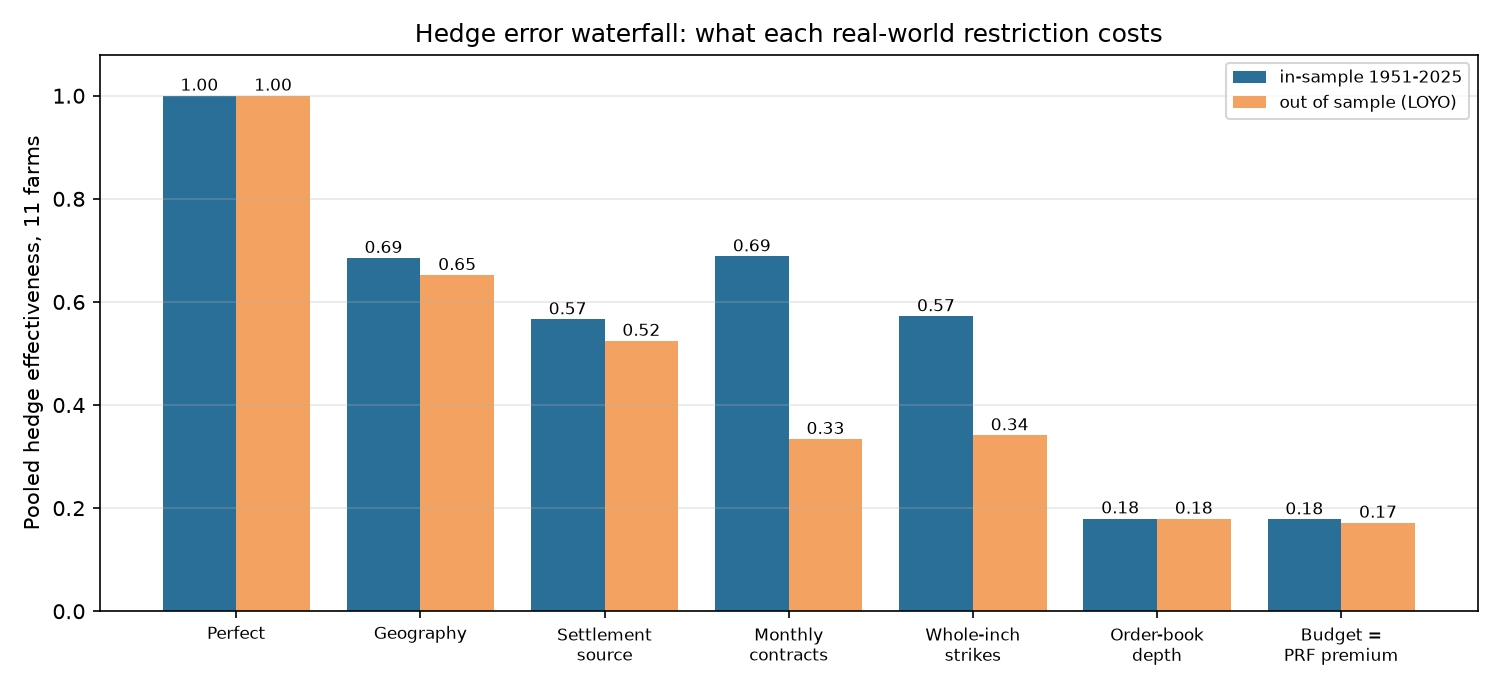
\includegraphics[width=0.9\textwidth]{m2_error_waterfall.png}
\caption{Pooled HE after each restriction, 11 farms, 1951--2025.}
\end{figure}

\textbf{Findings.} Geography is the largest loss ($-0.35$; the largest drop in 23 of 36 insured windows).
Settlement source costs a steady $-0.13$. Splitting PRF's two-month interval into monthly contracts costs
$-0.19$. Whole-inch binning costs nothing out of sample: finer strikes look 0.12 better in sample, but that
gain is overfitting. Order-book depth costs $-0.16$ (the largest loss in sample, $-0.39$). Once depth binds,
the capital constraint barely matters. Two thirds of the total loss (0.48 of 0.83) comes from paying on the
wrong rain, which no strike set or optimizer can fix.

\subsection{Exposures that cannot be replicated, and what would fix them (Evan)}

\begin{table}[H]\centering\small
\begin{tabularx}{\textwidth}{Yrrr}
\toprule
Contract set & Pooled HE out & Farms with HE $\ge 0.6$ & \$ per \$1 expected \\
\midrule
Today: monthly, whole-inch strikes & 0.34 & 0 of 11 & 1.10 \\
P1 monthly, half-inch strikes & 0.34 & 0 of 11 & 1.12 \\
P2 two-month total, 1-inch strikes & 0.48 & 2 of 11 & 1.13 \\
P3 two-month total, half-inch strikes & 0.47 & 2 of 11 & 1.14 \\
P4 binaries on the farm's grid index, 10-point steps & 0.98 & 11 of 11 & 1.20 \\
P5 same, 5-point steps & 0.99 & 11 of 11 & 1.20 \\
\bottomrule
\end{tabularx}
\caption{Proposed contracts (lowest-error hedge, no depth or budget limit).}
\end{table}

\textbf{Exposures that fail.} Only 3 of 36 insured windows reach HE 0.6 today (OKC spring and SGF fall);
21 are partial and 12 fail. The failures are summer convective or monsoon rain: every Albuquerque window,
Denver Jun--Sep, Tampa May--Jun, Springfield May--Jun, Dallas Aug--Sep, San Antonio Sep--Oct.

\textbf{What would fix them.} (1) \emph{Two-month contracts} (P2) need no new data source and improve 35 of 36
windows. They are the first thing to propose to the exchange. (2) \emph{Grid-index binaries} (P4) recover
almost everything, but they are PRF without the subsidy and need NOAA gridded data as a settlement source.
(3) \emph{Market mechanisms}: the busiest leg needs 5--28$\times$ today's sensible depth, and only 16\% of the
contracts could be filled. Hedging needs ladders listed 6--12 months ahead (today about 30 days), a
designated market maker on the drought side (rewarded depth fell 94\% when rewards ended), and pooled
orders through cooperatives or agents. Matching PRF's net benefit would need a subsidy of about \$44,600 a
year for the 11 farms.

%=====================================================================
\section{Building the App (Week 5)}

\subsection{Live-price backend (Jack)}

One function, \texttt{platform.quote}, serves the web app and the tests. It (1) maps the location to its
PRF grid and ranks the Kalshi stations within 25 miles of the nearest by out-of-sample fit; (2) builds the
PRF-style target for any chosen months; (3) prices each contract from Kalshi's public order-book API (cached
60\,s, with a saved-snapshot fallback), skipping levels more than 10\,\textcent{} above fair value; months not
yet listed are priced at fair value plus half a typical spread and flagged; (4) runs the optimizer for the
frontier and the recommended hedge; and (5) returns an order ticket with whole contracts, limit prices and
fees. Two rules came from live testing. Coverage starts with the next month that has not begun, because a
live test bought an in-progress November at 99\,\textcent{} when its price already reflected the rain so far.
The nearest station is not always the best: St.~Petersburg is nearer to the Tampa farms than Tampa, but has
only 17 years of record.

\subsection{Farmer screen (Maya)}

\begin{figure}[H]\centering
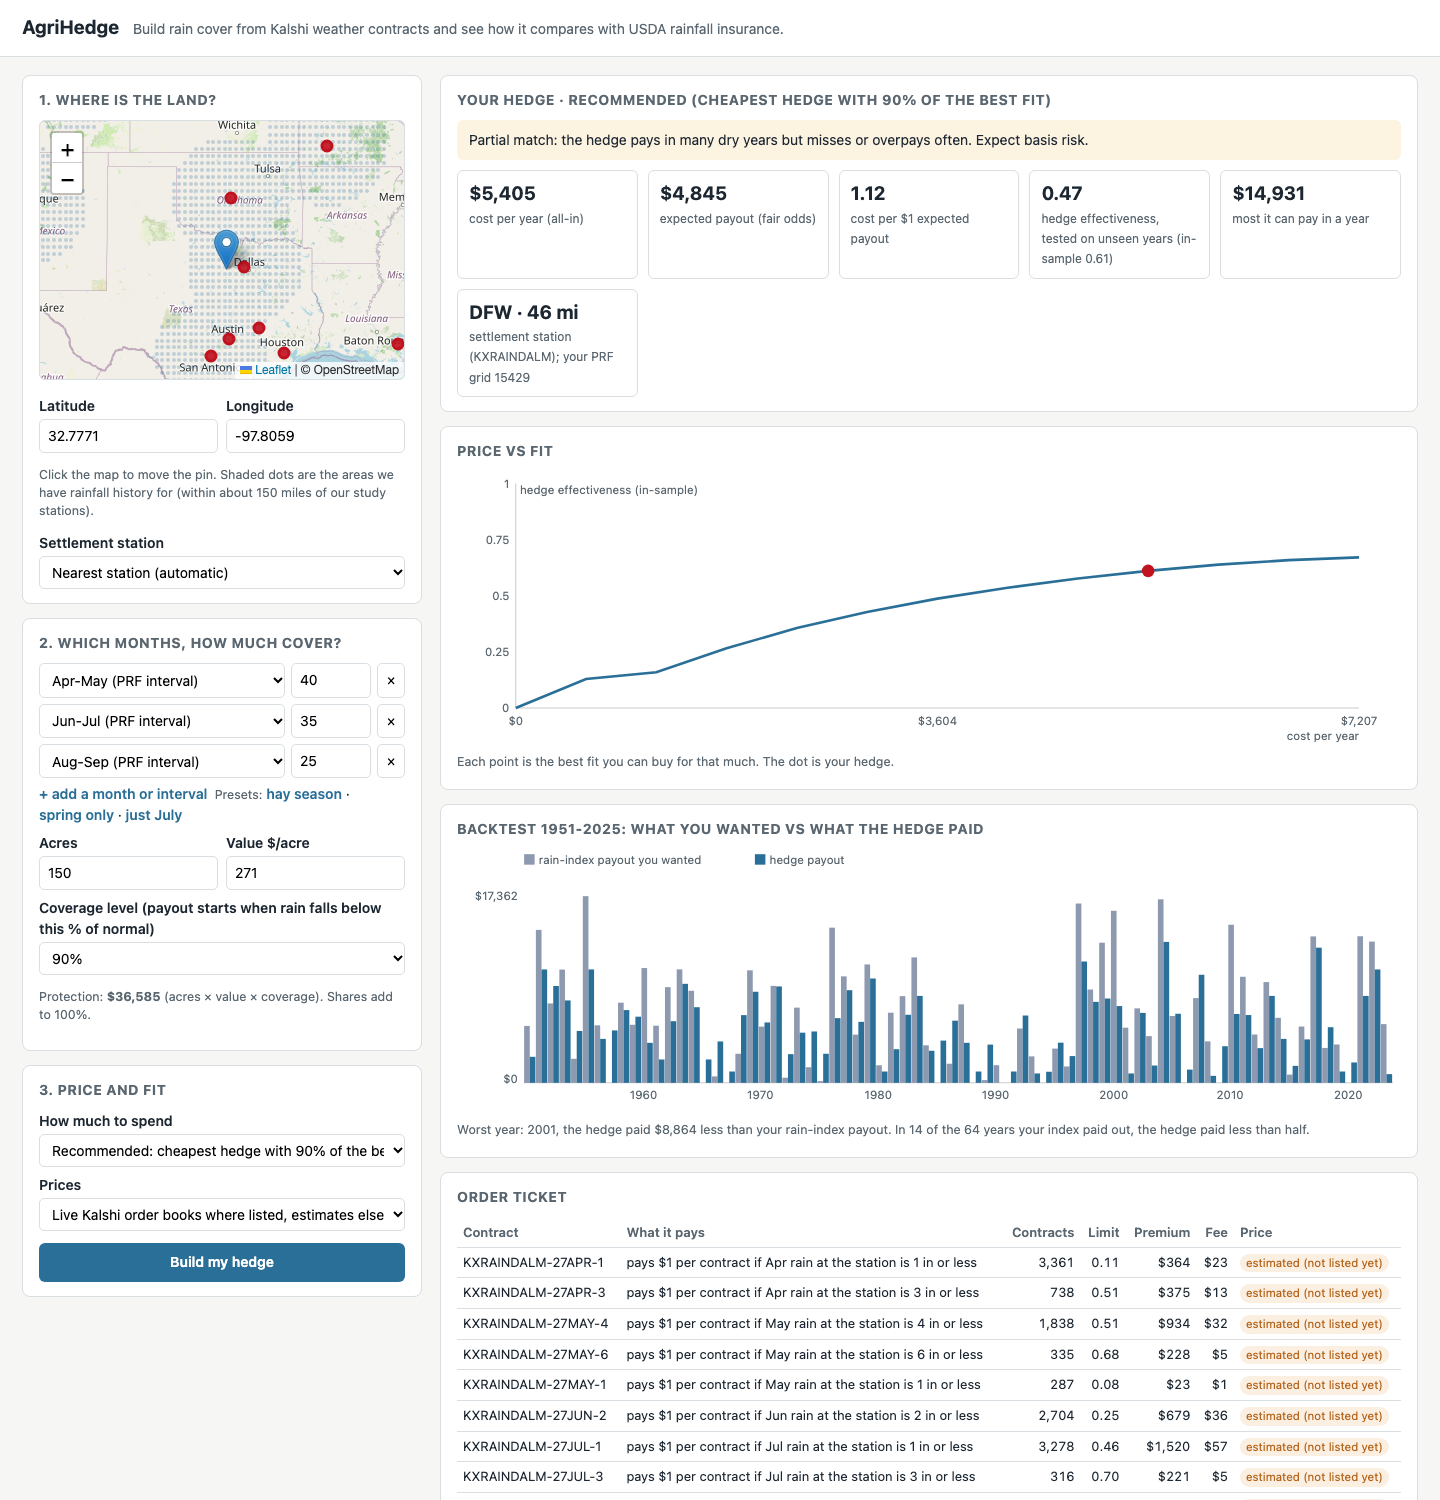
\includegraphics[width=\textwidth]{m2_app_screenshot.png}
\caption{The farmer screen: location, months and cover on the left; verdict, price-vs-fit frontier,
backtest, order ticket and PRF comparison on the right.}
\end{figure}

A farmer clicks the map (2,036 PRF grids around the 8 study stations are served), adds any PRF interval,
single month or three-month season with a share of protection, enters acres, value per acre and coverage
level, and chooses ``recommended'', ``best fit'' or a budget. The answer starts with a plain verdict (good,
partial or poor match, from out-of-sample HE) and shows the live market depth at the station.

\subsection{Testing the app against the USDA benchmark (Evan)}

Each farm typed its own location, PRF intervals, coverage and protection into the app (station
chosen automatically, estimated prices). Then a standard hay-season request was run at 150 random grids.

\begin{figure}[H]\centering
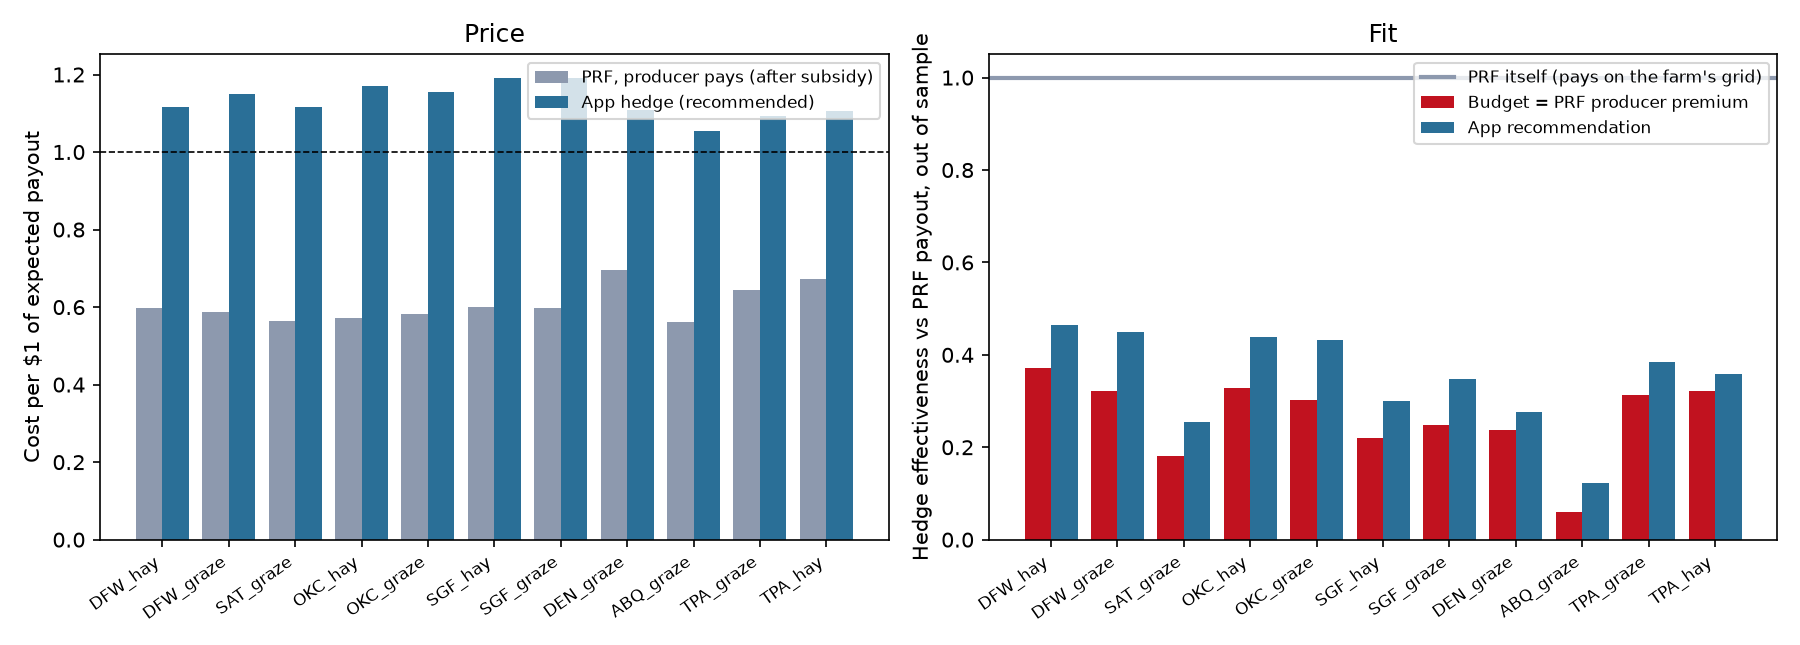
\includegraphics[width=\textwidth]{m2_app_vs_prf.png}
\caption{Left: cost per \$1 of expected payout, PRF (producer share) vs.\ the app's recommended hedge.
Right: out-of-sample HE against the PRF payout.}
\end{figure}

\begin{table}[H]\centering\small
\begin{tabularx}{\textwidth}{Yr}
\toprule
Measure (11 farms) & Value \\
\midrule
PRF producer premiums / app recommended hedges & \$55,994 / \$95,182 per year \\
Hedge cost $\div$ PRF producer premium, per farm & 1.56--1.97 (median 1.71) \\
Cost per \$1 expected payout: PRF producer / app hedge & \$0.56--0.70 / \$1.05--1.18 \\
Median HE out of sample: recommended / PRF-premium budget / lowest error & 0.38 / 0.30 / 0.37 \\
Years the hedge paid $<$ half of PRF, of years PRF paid & 2--11 of 50--68 per farm \\
Farm-years the hedge paid but PRF did not & 115 \\
Worst single-year shortfall & \$3,588 (SGF\_graze) to \$50,964 (ABQ\_graze) \\
App matches doc analysis (station, grid, cost) & 11 of 11; \$0.00 cost gap \\
App PRF premium estimate vs.\ real 2026 premium & median $+3\%$ ($-13\%$ to $+10\%$) \\
\bottomrule
\end{tabularx}
\caption{The app against the USDA PRF benchmark.}
\end{table}

\begin{figure}[H]\centering
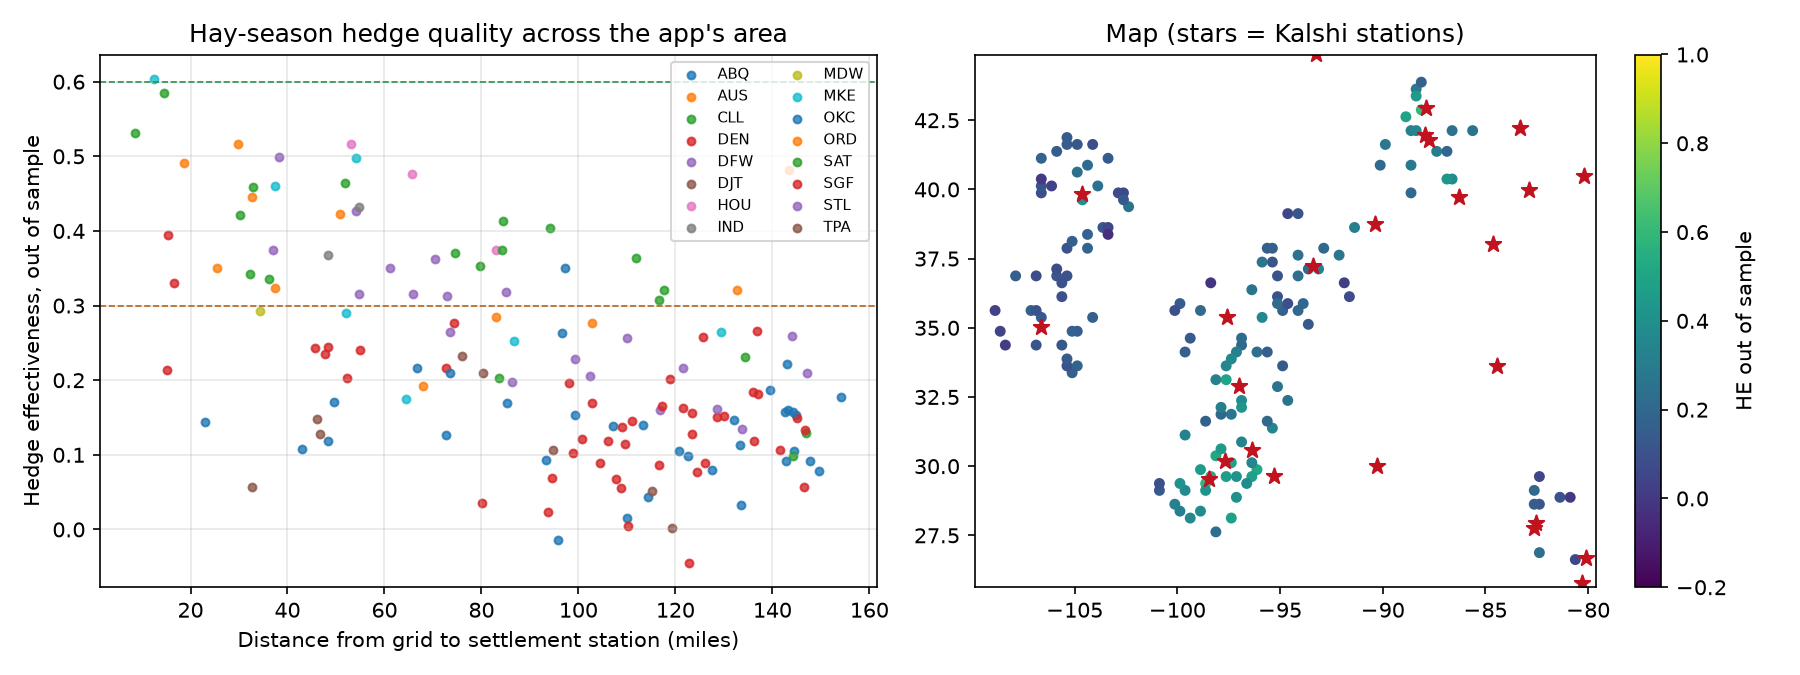
\includegraphics[width=\textwidth]{m2_app_sweep.png}
\caption{Hay-season hedge quality at 150 random grids: out-of-sample HE vs.\ distance to the settlement
station (left) and on a map (right).}
\end{figure}

\textbf{Findings.} The app is correct, and its answer is sobering. Hedging PRF's own intervals costs about 1.7$\times$ what
PRF costs the farmer and copies a bit over a third of PRF's swings. In 115 farm-years it paid when PRF did
not, and those false alarms are what make it expensive. Distance decides who can use it: median HE is 0.47
within 25 miles, 0.35 at 25--50, and 0.15 beyond 100 miles. (The app now recommends the cheapest hedge with
95\% of the best fit, which did best on unseen years across 44 cases.) With only 7.4\% of US PRF grids within 50 miles of a Kalshi rain
station (Milestone I), a useful hedge reaches a small minority of PRF land. On 2026-11-05 no month beyond
the one in progress was listed, so every order for a real season was correctly flagged as estimated.

%=====================================================================
\section{Complementing PRF (refinements from our Milestone I update)}

Our Milestone I update said we would complement PRF rather than replace it, by targeting cover above
PRF's 90\% cap, uncovered months and too much rain. It also said we would look beyond binary payouts and
backtest on the index USDA actually paid (CPC), with NCEI for forward results.

\begin{figure}[H]\centering
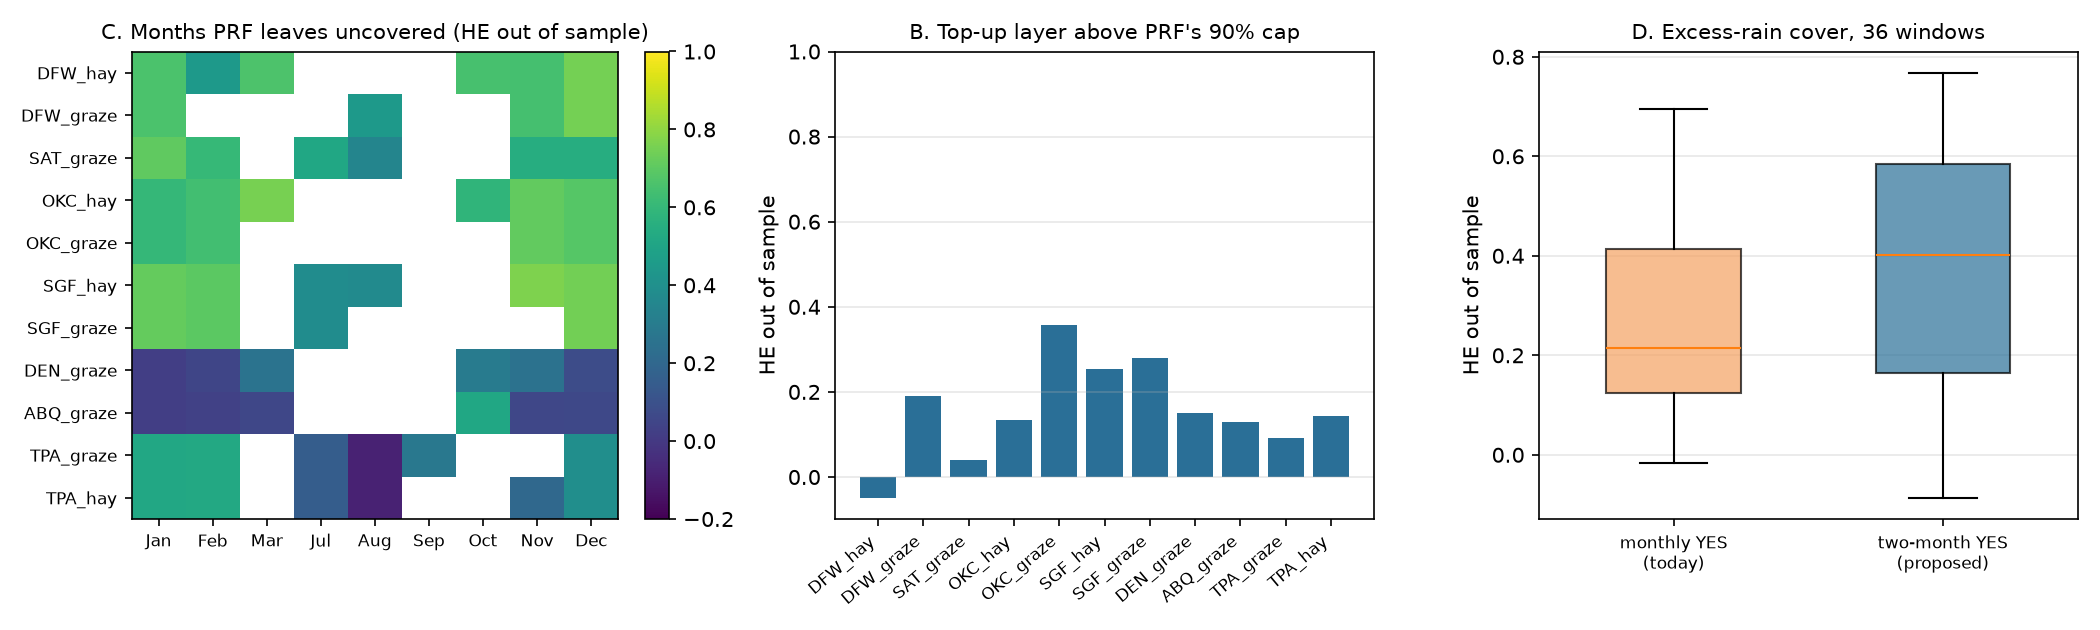
\includegraphics[width=\textwidth]{m2_prf_gaps.png}
\caption{Left: out-of-sample HE of single-month cover for months outside each farm's PRF intervals.
Middle: a top-up layer above PRF's 90\% cap. Right: excess-rain cover with monthly vs.\ two-month YES contracts.}
\end{figure}

\begin{table}[H]\centering\small
\begin{tabularx}{\textwidth}{Yrr}
\toprule
Gap PRF leaves & Median HE in & Median HE out of sample \\
\midrule
Uncovered months, single-month cover at 90\% (60 farm-months) & -- & 0.52 (26 of 60 $\ge 0.6$) \\
Top-up layer above PRF's 90\% cap (11 farms) & 0.40 & 0.14 \\
Excess rain ($>130\%$ of normal), today's monthly YES (36 windows) & 0.47 & 0.22 \\
Excess rain, proposed two-month YES (36 windows) & 0.70 & 0.40 \\
\midrule
PRF itself, CPC as paid vs.\ NCEI, 1969--2025 (lowest error / knee) & -- & 0.20 vs.\ 0.28 / 0.26 vs.\ 0.27 \\
\bottomrule
\end{tabularx}
\caption{Where event contracts can complement PRF.}
\end{table}

\textbf{Findings.} Cool-season frontal rain spreads evenly over a region, so the airport gauge tracks the
farm in the months PRF leaves open (December 0.68, November 0.65, January 0.60). That is the strongest use
of today's contracts we found. The value is mainly for winter pasture, stock water and winter wheat, because
warm-season forage responds little to winter rain. A top-up above 90\% pays a little in nearly every year and
copies poorly. Excess-rain cover works only with two-month contracts, which strengthens the case for them.
On payouts beyond binaries: contracts paying the PRF formula linearly on the station gauge or station grid
index reach 0.52--0.65 (Section 1.2). Grid-index binaries reach 0.98. So what matters is \emph{what} a
contract settles on, not the payout shape. Backtesting on the CPC index USDA actually paid gives slightly
lower out-of-sample HE than NCEI on the same years. The 90\% knee closes most of that gap. Temperature risk
(``if time permits'') is left for Milestone III.

%=====================================================================
\section{Showcase: the PRF Companion}

Sections 1--3 point to one product. Kalshi rain contracts are a poor \emph{substitute} for PRF, but a good
\emph{complement} in the months PRF leaves open. The app's PRF Companion tab does exactly that:
\begin{enumerate}
  \item The rancher enters a location and the PRF intervals they insure.
  \item Each month PRF leaves open is scored by out-of-sample HE.
  \item Months at 0.5 or above are recommended and combined into one Kalshi order.
  \item A 1951--2025 backtest shows the companion's payouts next to what PRF paid.
\end{enumerate}

\begin{figure}[H]\centering
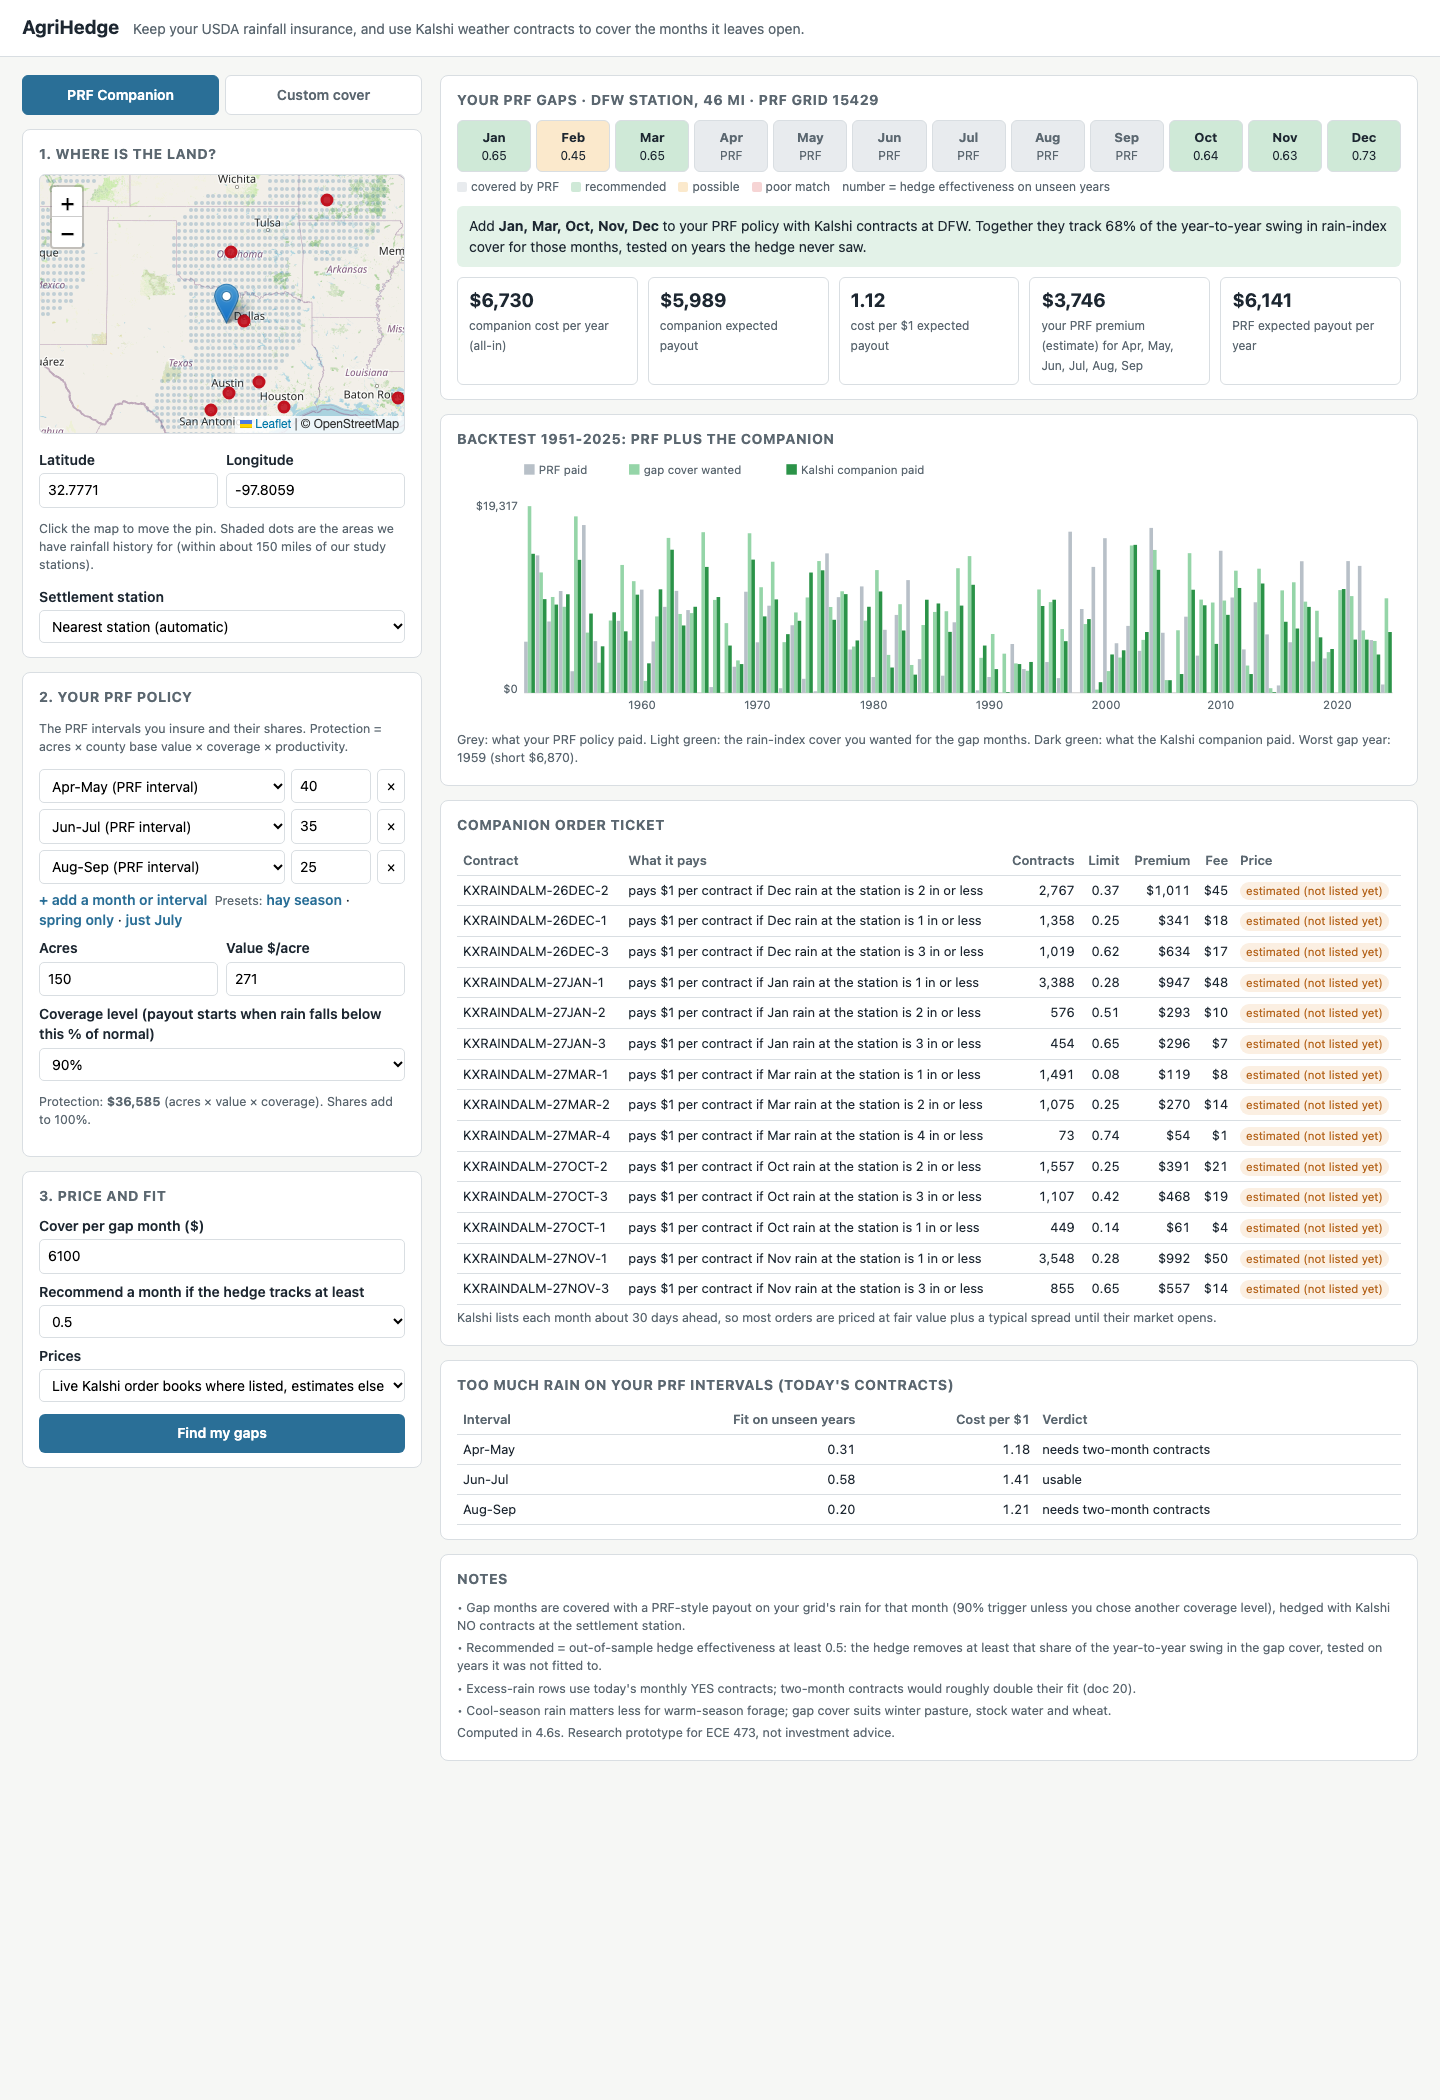
\includegraphics[width=\textwidth]{m2_companion_screenshot.png}
\caption{The PRF Companion for the Dallas hay farm (PRF on Apr--Sep). The month strip shows the recommended gap
months (green), with their out-of-sample HE. Below it: the package, the backtest of PRF plus the companion,
and the order ticket.}
\end{figure}

\begin{figure}[H]\centering
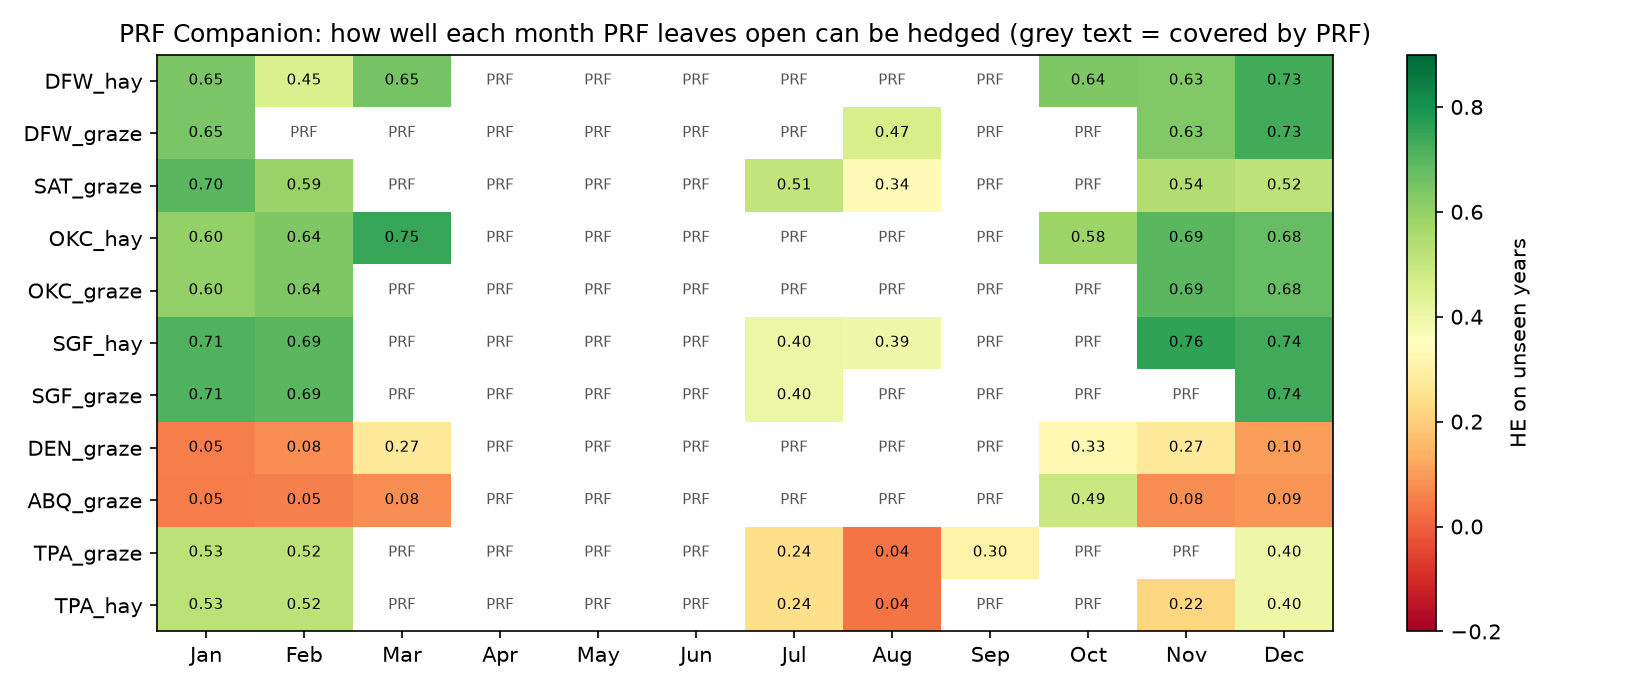
\includegraphics[width=\textwidth]{m2_companion_farms.png}
\caption{Out-of-sample HE of a Kalshi hedge for every month each farm's PRF policy leaves open.}
\end{figure}

\begin{table}[H]\centering\small
\begin{tabularx}{\textwidth}{Yrr}
\toprule
Measure & PRF Companion & Hedging PRF's own intervals \\
\midrule
Farms where it is recommended & 9 of 11 & -- \\
Median HE out of sample (leave one year out) & 0.66 & 0.38 \\
Holdout: months chosen and fit on 1951--2000, scored on 2001--2025 & 0.61 & 0.23 \\
Random grids with a useful result (60 grids / 150 grids) & 60\% with $\ge 1$ month & 1\% with HE $\ge 0.6$ \\
Cost per \$1 of expected payout (median) & \$1.10 & \$1.12 \\
\bottomrule
\end{tabularx}
\caption{The companion against hedging PRF itself.}
\end{table}

\textbf{Findings.} December, November and January carry the companion: 7 of 11, 6 of 9 and 9 of 11 of those
farm-months are recommended. Summer months almost never are. Picking months and fitting on 1951--2000 only,
the companion still scores 0.61 on 2001--2025, so the result is not an artifact of choosing on the test
years. Combining several nearby stations does not help, because Kalshi stations are too sparse; only the Tampa
farms gain (0.37 to 0.43). Caveats: winter rain matters less for warm-season forage, so the value is greatest
for winter pasture, winter wheat and stock water. Each month is listed only about 30 days ahead, so orders are
placed month by month.

\textbf{What the rest of the project builds on.} The companion is the platform the remaining work expands:
\begin{itemize}
  \item wet-side (excess-rain) cover;
  \item a mock two-month market to demonstrate our contract proposal;
  \item national coverage for all 38 Kalshi rain stations;
  \item hedging modeled forage loss instead of the PRF formula;
  \item temperature risk;
  \item order placement in Kalshi's demo environment.
\end{itemize}

%=====================================================================
\section{Synthesis and Next Steps}

The platform works, and it gives a farmer an honest answer. That answer is mostly ``not yet''. With
today's contracts, the best hedge near a station removes about a third of PRF's payout variance out of
sample, costs about \$1.10 per \$1 of expected payout against \$0.61 for subsidized PRF, and cannot be
filled from current order books. Strike binning, the problem Milestone I flagged first, turns out not to
matter. The binding problems are where the rain is measured, how long the contract window is, and who is
on the other side of the trade. The constructive results are a ranked list of fixes: two-month contracts
(no new data needed), seasonal listing, a drought-side market maker, and, as the end point, contracts on a
gridded rain index. As our Milestone I update proposed, the tool is most useful as a complement to PRF.
The PRF Companion makes that concrete: in the cool-season months PRF leaves open, a Kalshi hedge near a
station tracks the farm's rain well on years it never saw (0.61). That is the base the rest of the project
builds on.

\textbf{Reproducibility.} Code and data: \url{https://github.com/Belugaluga2/ECE473-Project} (docs 15--21; demo guide \texttt{docs/DEMO.md}).
\texttt{python scripts/run\_optimizer.py}, \texttt{run\_error\_budget.py}, \texttt{run\_app\_test.py
--live}, \texttt{run\_prf\_gaps.py}, \texttt{run\_companion\_study.py}, \texttt{run\_companion\_holdout.py};
app: \texttt{python scripts/run\_app.py} (\texttt{?demo} runs the companion). 352 automated tests (19 new for Milestone II).

\end{document}
